\documentclass[
  doc,
  longtable,
  nolmodern,
  notxfonts,
  notimes,
  colorlinks=true,linkcolor=blue,citecolor=blue,urlcolor=blue]{apa7}

\usepackage{amsmath}
\usepackage{amssymb}




\RequirePackage{longtable}
\RequirePackage{threeparttablex}

\makeatletter
\renewcommand{\paragraph}{\@startsection{paragraph}{4}{\parindent}%
	{0\baselineskip \@plus 0.2ex \@minus 0.2ex}%
	{-.5em}%
	{\normalfont\normalsize\bfseries\typesectitle}}

\renewcommand{\subparagraph}[1]{\@startsection{subparagraph}{5}{0.5em}%
	{0\baselineskip \@plus 0.2ex \@minus 0.2ex}%
	{-\z@\relax}%
	{\normalfont\normalsize\bfseries\itshape\hspace{\parindent}{#1}\textit{\addperi}}{\relax}}
\makeatother




\usepackage{longtable, booktabs, multirow, multicol, colortbl, hhline, caption, array, float, xpatch}
\setcounter{topnumber}{2}
\setcounter{bottomnumber}{2}
\setcounter{totalnumber}{4}
\renewcommand{\topfraction}{0.85}
\renewcommand{\bottomfraction}{0.85}
\renewcommand{\textfraction}{0.15}
\renewcommand{\floatpagefraction}{0.7}

\usepackage{tcolorbox}
\tcbuselibrary{listings,theorems, breakable, skins}
\usepackage{fontawesome5}

\definecolor{quarto-callout-color}{HTML}{909090}
\definecolor{quarto-callout-note-color}{HTML}{0758E5}
\definecolor{quarto-callout-important-color}{HTML}{CC1914}
\definecolor{quarto-callout-warning-color}{HTML}{EB9113}
\definecolor{quarto-callout-tip-color}{HTML}{00A047}
\definecolor{quarto-callout-caution-color}{HTML}{FC5300}
\definecolor{quarto-callout-color-frame}{HTML}{ACACAC}
\definecolor{quarto-callout-note-color-frame}{HTML}{4582EC}
\definecolor{quarto-callout-important-color-frame}{HTML}{D9534F}
\definecolor{quarto-callout-warning-color-frame}{HTML}{F0AD4E}
\definecolor{quarto-callout-tip-color-frame}{HTML}{02B875}
\definecolor{quarto-callout-caution-color-frame}{HTML}{FD7E14}

\newlength\Oldarrayrulewidth
\newlength\Oldtabcolsep


\usepackage{hyperref}




\providecommand{\tightlist}{%
  \setlength{\itemsep}{0pt}\setlength{\parskip}{0pt}}
\usepackage{longtable,booktabs,array}
\usepackage{calc} % for calculating minipage widths
% Correct order of tables after \paragraph or \subparagraph
\usepackage{etoolbox}
\makeatletter
\patchcmd\longtable{\par}{\if@noskipsec\mbox{}\fi\par}{}{}
\makeatother
% Allow footnotes in longtable head/foot
\IfFileExists{footnotehyper.sty}{\usepackage{footnotehyper}}{\usepackage{footnote}}
\makesavenoteenv{longtable}

\usepackage{graphicx}
\makeatletter
\def\maxwidth{\ifdim\Gin@nat@width>\linewidth\linewidth\else\Gin@nat@width\fi}
\def\maxheight{\ifdim\Gin@nat@height>\textheight\textheight\else\Gin@nat@height\fi}
\makeatother
% Scale images if necessary, so that they will not overflow the page
% margins by default, and it is still possible to overwrite the defaults
% using explicit options in \includegraphics[width, height, ...]{}
\setkeys{Gin}{width=\maxwidth,height=\maxheight,keepaspectratio}
% Set default figure placement to htbp
\makeatletter
\def\fps@figure{htbp}
\makeatother


% definitions for citeproc citations
\NewDocumentCommand\citeproctext{}{}
\NewDocumentCommand\citeproc{mm}{%
  \begingroup\def\citeproctext{#2}\cite{#1}\endgroup}
\makeatletter
 % allow citations to break across lines
 \let\@cite@ofmt\@firstofone
 % avoid brackets around text for \cite:
 \def\@biblabel#1{}
 \def\@cite#1#2{{#1\if@tempswa , #2\fi}}
\makeatother
\newlength{\cslhangindent}
\setlength{\cslhangindent}{1.5em}
\newlength{\csllabelwidth}
\setlength{\csllabelwidth}{3em}
\newenvironment{CSLReferences}[2] % #1 hanging-indent, #2 entry-spacing
 {\begin{list}{}{%
  \setlength{\itemindent}{0pt}
  \setlength{\leftmargin}{0pt}
  \setlength{\parsep}{0pt}
  % turn on hanging indent if param 1 is 1
  \ifodd #1
   \setlength{\leftmargin}{\cslhangindent}
   \setlength{\itemindent}{-1\cslhangindent}
  \fi
  % set entry spacing
  \setlength{\itemsep}{#2\baselineskip}}}
 {\end{list}}
\usepackage{calc}
\newcommand{\CSLBlock}[1]{\hfill\break\parbox[t]{\linewidth}{\strut\ignorespaces#1\strut}}
\newcommand{\CSLLeftMargin}[1]{\parbox[t]{\csllabelwidth}{\strut#1\strut}}
\newcommand{\CSLRightInline}[1]{\parbox[t]{\linewidth - \csllabelwidth}{\strut#1\strut}}
\newcommand{\CSLIndent}[1]{\hspace{\cslhangindent}#1}





\usepackage{newtx}

\defaultfontfeatures{Scale=MatchLowercase}
\defaultfontfeatures[\rmfamily]{Ligatures=TeX,Scale=1}





\title{Statistical Inconsistencies in Experimental Linguistics}


\shorttitle{Statistical Inconsistencies}


\usepackage{etoolbox}








\authorsnames{Timo B. Roettger,Dara Leonard Jenssen Etemady}





\affiliation{
{Department of Linguistics \& Scandinavian Studies, University of Oslo}}




\leftheader{Roettger and Etemady}



\abstract{Lorem ipsum dolor sit amet, consectetur adipiscing elit, sed
do eiusmod tempor incididunt ut labore et dolore magna aliqua. Ut enim
ad minim veniam, quis nostrud exercitation ullamco laboris nisi ut
aliquip ex ea commodo consequat. Duis aute irure dolor in reprehenderit
in voluptate velit esse cillum dolore eu fugiat nulla pariatur.
Excepteur sint occaecat cupidatat non proident, sunt in culpa qui
officia deserunt mollit anim id est laborum.}

\keywords{statistics, statcheck, reproducibility}

\authornote{\par{\addORCIDlink{Timo B. Roettger}{0000-0000-0000-0001}} 
\par{ }
\par{       }
\par{Correspondence concerning this article should be addressed to Timo
B. Roettger, Email: timo.roettger@gmail.com}
}

\makeatletter
\let\endoldlt\endlongtable
\def\endlongtable{
\hline
\endoldlt
}
\makeatother

\urlstyle{same}



\makeatletter
\@ifpackageloaded{caption}{}{\usepackage{caption}}
\AtBeginDocument{%
\ifdefined\contentsname
  \renewcommand*\contentsname{Table of contents}
\else
  \newcommand\contentsname{Table of contents}
\fi
\ifdefined\listfigurename
  \renewcommand*\listfigurename{List of Figures}
\else
  \newcommand\listfigurename{List of Figures}
\fi
\ifdefined\listtablename
  \renewcommand*\listtablename{List of Tables}
\else
  \newcommand\listtablename{List of Tables}
\fi
\ifdefined\figurename
  \renewcommand*\figurename{Figure}
\else
  \newcommand\figurename{Figure}
\fi
\ifdefined\tablename
  \renewcommand*\tablename{Table}
\else
  \newcommand\tablename{Table}
\fi
}
\@ifpackageloaded{float}{}{\usepackage{float}}
\floatstyle{ruled}
\@ifundefined{c@chapter}{\newfloat{codelisting}{h}{lop}}{\newfloat{codelisting}{h}{lop}[chapter]}
\floatname{codelisting}{Listing}
\newcommand*\listoflistings{\listof{codelisting}{List of Listings}}
\makeatother
\makeatletter
\makeatother
\makeatletter
\@ifpackageloaded{caption}{}{\usepackage{caption}}
\@ifpackageloaded{subcaption}{}{\usepackage{subcaption}}
\makeatother

% From https://tex.stackexchange.com/a/645996/211326
%%% apa7 doesn't want to add appendix section titles in the toc
%%% let's make it do it
\makeatletter
\xpatchcmd{\appendix}
  {\par}
  {\addcontentsline{toc}{section}{\@currentlabelname}\par}
  {}{}
\makeatother

\begin{document}

\maketitle


\setcounter{secnumdepth}{-\maxdimen} % remove section numbering

\setlength\LTleft{0pt}


\section{1. Introduction}\label{introduction}

What we know about human language and its cognitive underpinnings is
often informed by experimental data, data based on which researchers
draw theoretically relevant inferences using common statistical
frameworks. This inference should be transparent in order for other
researchers to critically evaluate the inference process and potentially
detect and correct human errors. In the recent years, the quantitative
sciences have seen repeated calls to become more transparent and
reproducible by sharing data and statistical protocols
(\citeproc{ref-arvan2022reproducibility}{Arvan et al., 2022};
\citeproc{ref-laurinavichyute2022share}{Laurinavichyute et al., 2022};
\citeproc{ref-roettger2019researcher}{Roettger, 2019}), sharing of
statistical protocols is still rare across the language sciences
(\citeproc{ref-bochynska2023reproducible}{Bochynska et al., 2023}). If
statistical procedures cannot be critically evaluated, human errors
might be left undetected and thus remain uncorrected in the publication
record. If these errors affect the decision procedure of the analysis,
i.e.~whether a hypothesis is rejected or accepted, these errors might
lead to -at best- overconfident, -at worst- false theoretical
conclusions. The present paper will present evidence that the published
literature in experimental linguistics contains a concerning amount of
statistical errors, a state of affairs which warrants more rigorous data
sharing practices.

\section{2. Statistal reporting
inconsistencies}\label{statistal-reporting-inconsistencies}

The null-hypothesis significance testing (NHST) framework is, to date,
the most dominant statistical framework that researchers use to test
hypotheses in the language sciences
(\citeproc{ref-sondereggera2024advancements}{Sonderegger \& Sóskuthy,
2024}). These statistical tests are reported in specific formats which
usually contain a test statistic, the degrees of freedom of that test
(if applicable), and the p-value, representing the probability of
observing the data (or more extreme data) given the null hypothesis
(i.e.~given that the test statistic is zero) (see example 1):\\
(1) F(1, 66) = 3.88, p \textless{} .05\\
Since data and statistical protocol sharing remains rare across the
language sciences (\citeproc{ref-bochynska2023reproducible}{Bochynska et
al., 2023}), interested readers are left with trusting the authors that
the statistical analysis is run and reported correctly. Whether that
trust is warranted can be assessed, however. The three sets of indices
in (1) have a clearly defined mathematical relationship and can thus be
checked for consistency. An F test with the specified degrees of freedom
and a test-statistic of 3.88 should result in a p-value of 0.053 which
is larger, not smaller, than 0.05. Thus, something is wrong with the
statistical report in (1). Possible reasons for this inconsistency are
manifold: It could be a typo of the comparison sign, i.e.~the authors
meant to use \texttt{=} or \texttt{\textgreater{}} rather than
\texttt{\textless{}}. Alternatively, any of the numbers could be a typo.
Sometimes an error might indicate erroneous rounding (e.g.~0.057 being
rounded down to 0.05). Other times, human error along the data
analytical pipeline might have caused an error down the line. Without
access to data and scripts, it remains unclear to the reader, what has
caused the inconsistency. Such inconsistencies can be particularly
concerning if the calculated p-value and the reported p-values are not
on the same side of the alpha threshold. In NHST, p-values below a
conventionalized alpha threshold, most commonly 0.05, are interpreted as
evidence that the data are sufficiently inconsistent with the null
hypothesis (significant). p-values above that threshold are considered
consistent with the null hypothesis and practically lead to rejecting
the alternative hypothesis (not significant). In (1) above, the reported
p-value suggest a significant result, the p-value derived from the
degrees of freedom and the test statistic suggest a non-significant
result. In the following we refer to these inconsistencies as ``decision
inconsistency''.

This form of inconsistency assessment can be automatically assessed if
statistical tests are reported in an unambiguous format. Recently, a
series of studies used such automatic assessments to evaluate the
prevalence of inconsistent statistical reporting across different
disciplines (\citeproc{ref-buckley2023estimating}{Buckley et al., 2023};
\citeproc{ref-green2018statcheck}{Green et al., 2018};
\citeproc{ref-gross2021fidelity}{Groß, 2021}; e.g.
\citeproc{ref-nuijten2016prevalence}{Nuijten et al., 2016};
\citeproc{ref-nuijten2020statcheck}{Nuijten \& Polanin, 2020}). For
example, looking at over 250000 p-values published in major psychology
journals, Nuijten et al. (\citeproc{ref-nuijten2016prevalence}{2016})
found that around 50\% of the articles with statistical results
contained at least one inconsistencies and around 12.5\% contained at
least one ``decision inconsistency''.

To assess the prevalence of statistical-reporting inconsistencies in
experimental linguistics, the present paper conceptually replicates
Nuijten et al. (\citeproc{ref-nuijten2016prevalence}{2016}) and assesses
over 39000 p-values reported in eight experimental linguistic journals
published between 2000 and 2023. We further assess whether the rate of
inconsistency differs across journals, whether that rate has changed
over the course of the last 20 years and whether there is evidence for
bias in these statistical-reporting inconsistencies. We discuss the
results and offer concrete recommendations for authors, reviewers, and
editors to tackle this problem.

\section{3. Method}\label{method}

All quantitative analyses were conducted using R {[}{]} and the r
packages {[}LIST ALL PACKAGES from 01\_Analysis.R and add to
references{]}

\subsection{3.1. Statcheck}\label{statcheck}

We used the R package statcheck (Version 1.4.1-beta.2,
\citeproc{ref-nuijten2023statcheck}{Nuijten \& Epskamp, 2023}) to
automatically detect statistical-reporting inconsistencies. Statcheck
works as follows: After converting pdf or html articles to plain text,
statcheck searches for specific strings that correspond to a NHST
result, using ``regular expressions''. That way, statcheck can detect
results of t tests, F tests, Z tests, χ2 tests, correlation tests, and Q
tests as long as the test result fulfills three conditions: (a) the test
result is reported completely including the test statistic, degrees of
freedom (if applicable), and the p-value; (b) the test result is in the
body of the text, i.e.~it usually misses results reported in tables; and
(c) the test result is reported in American Psychological Association
style (APA, 2019). Given these constraints, statcheck is estimated to
detect roughly 60\% of all reported NHST results
(\citeproc{ref-nuijten2016prevalence}{Nuijten et al., 2016}) Statcheck
uses the reported test statistic and degrees of freedom to recalculate
the p-value, compares the reported and recalculated p-values and, if
there is a mismatch, reports a comparison as an ``inconsistency.'' The
algorithm takes into account that tests might have been performed as
one-tailed by identifying the search strings ``one-tailed,''
``one-sided,'' or ``directional''. Moreover, statcheck counts p = .000
and p \textless{} .000 as inconsistent as p-values of exactly zero are
mathematically impossible and the APA manual
(\citeproc{ref-APA2020}{American Psychological Association, 2020})
advises to report very small p-values as p \textless{} .001. Validity
checks suggest that inter rater reliability between manual coding and
statcheck is high, i.e.~0.76 for inconsistencies and 0.89 for decision
inconsistencies (\citeproc{ref-nuijten2016prevalence}{Nuijten et al.,
2016}). The overall accuracy of statcheck is estimated between 96.2\% to
99.9\% (\citeproc{ref-nuijten2017validity}{Nuijten et al., 2017}). We
thus consider statcheck a valid, but rough proxy of statistical
reporting inconsistencies.

\subsection{3.2. Sample}\label{sample}

Focusing on experimental linguistic research, we started with Kobrock
and Roettger (\citeproc{ref-kobrock2023assessing}{2023}) as a point of
departure who list 100 linguistic journals that had at least a hundred
articles published at the time of assessment (2021) and a high ratio of
articles containing the term ``experiment* in title, abstract or
keywords. Out of these 100 journals, we selected all journals with at
least 10\% of articles containing the search string''experiment*``. Out
of the remaining 37 journals, we selected those journals that urged APA
formatting either in the main body of the text or specifically regarding
statistics in the author guidelines, resulting in nine remaining
journals. Moreover, to download the pdfs, the articles had to be either
accessible to us through our library license, or open access, resulting
in a final list of eight journals: Applied Psycholinguistics (APS),
Bilingualism: Language and Cognition (BLC), Linguistic Approaches to
Bilingualism (LAB), Language and Speech (LaS), Language Learning and
Techology (LLT), Journal of Language and Social Psychology (LSP),
Journal of Child Language (JCL), and Studies in Second Language
Acquisition (SLA).

We included only original research articles within the publication years
of 2000-2023, excluding any book reviews, response articles,
commentaries, editorials, corrigenda, errata, advertisements, etc.
Articles from LAB spanned 2011-2023, while the rest spanned 2000-2023.
This procedure resulted in 5804 research articles. All 5804 articles
were submitted to analysis, using Statcheck v1.5.0. 157 articles were
not analyzable by statcheck, and thus had to be removed from the pool,
likely related to issues with rendering the Chi-Squared symbol being
erroneously converted from .pdf to .txt.

\subsection{3.3. Data availability
statement}\label{data-availability-statement}

All derived data and corresponding R scripts are publicly available
here: LINK. The original journal articles cannot be bulk-shared due to
distribution restrictions by the publishers. NEED TO FIGURE OUT A WAY

\section{4. Results}\label{results}

\subsection{4.1 Prevalence of
inconsistencies}\label{prevalence-of-inconsistencies}

The results are summarized in Table~\ref{tbl-summary}. Out of 5804
articles, 3059 articles contained statistical tests that statcheck could
assess (53\%), amounting to 39532 assessable p-values. 5166 p-values
were flagged as inconsistent (13.1\%) and 655 of which were considered
decisions inconsistencies (1.7\%) (see Table~\ref{tbl-summary}).

\begin{table}

{\caption{{Summary. Applied Psycholinguistics (APS), Bilingualism:
Language and Cognition (BLC), Linguistic Approaches to Bilingualism
(LAB), Language and Speech (LaS), Language Learning and Techology (LLT),
Journal of Language and Social Psychology (LSP), Journal of Child
Language (JCL), and Studies in Second Language Acquisition
(SLA).}{\label{tbl-summary}}}}

\begin{longtable}[]{@{}
  >{\raggedright\arraybackslash}p{(\columnwidth - 10\tabcolsep) * \real{0.0755}}
  >{\raggedleft\arraybackslash}p{(\columnwidth - 10\tabcolsep) * \real{0.1698}}
  >{\raggedleft\arraybackslash}p{(\columnwidth - 10\tabcolsep) * \real{0.1887}}
  >{\raggedleft\arraybackslash}p{(\columnwidth - 10\tabcolsep) * \real{0.1792}}
  >{\raggedleft\arraybackslash}p{(\columnwidth - 10\tabcolsep) * \real{0.1509}}
  >{\raggedleft\arraybackslash}p{(\columnwidth - 10\tabcolsep) * \real{0.2358}}@{}}
\toprule\noalign{}
\begin{minipage}[b]{\linewidth}\raggedright
Journal
\end{minipage} & \begin{minipage}[b]{\linewidth}\raggedleft
eligible articles
\end{minipage} & \begin{minipage}[b]{\linewidth}\raggedleft
assessible articles
\end{minipage} & \begin{minipage}[b]{\linewidth}\raggedleft
assessible results
\end{minipage} & \begin{minipage}[b]{\linewidth}\raggedleft
inconsistencies
\end{minipage} & \begin{minipage}[b]{\linewidth}\raggedleft
decision inconsistencies
\end{minipage} \\
\midrule\noalign{}
\endhead
\bottomrule\noalign{}
\endlastfoot
APS & 953 & 690 & 9570 & 1368 & 170 \\
BLC & 964 & 610 & 9093 & 1161 & 120 \\
JCL & 1109 & 529 & 6240 & 750 & 69 \\
LAB & 471 & 133 & 1719 & 234 & 25 \\
LLT & 421 & 111 & 919 & 201 & 61 \\
LSP & 695 & 376 & 4320 & 429 & 60 \\
LaS & 598 & 363 & 4717 & 552 & 86 \\
SLA & 593 & 247 & 2954 & 471 & 64 \\
Total & 5804 & 3059 & 39532 & 5166 & 655 \\
\end{longtable}

\end{table}

The proportion of inconsistencies ranged from 10 to 22\% across journals
(1 to 7\% for decisions inconsistencies) (see
Figure~\ref{fig-stacked-bar}). These rates appear to be stable across
year of publication (see Figure~\ref{fig-year-prop}). On average, 50\%
of assessable articles contained one or more inconsistencies (journals
range from 43 to 56\%) and 13\% contained one or more decisions
inconsistencies (journals range from 11 to 15\%).

\begin{figure}[H]

\caption{\label{fig-stacked-bar}Proportion of articles containing at
least one inconsistency / decision inconsistency. Applied
Psycholinguistics (APS), Bilingualism: Language and Cognition (BLC),
Linguistic Approaches to Bilingualism (LAB), Language and Speech (LaS),
Language Learning and Techology (LLT), Journal of Language and Social
Psychology (LSP), Journal of Child Language (JCL), and Studies in Second
Language Acquisition (SLA).}

\centering{

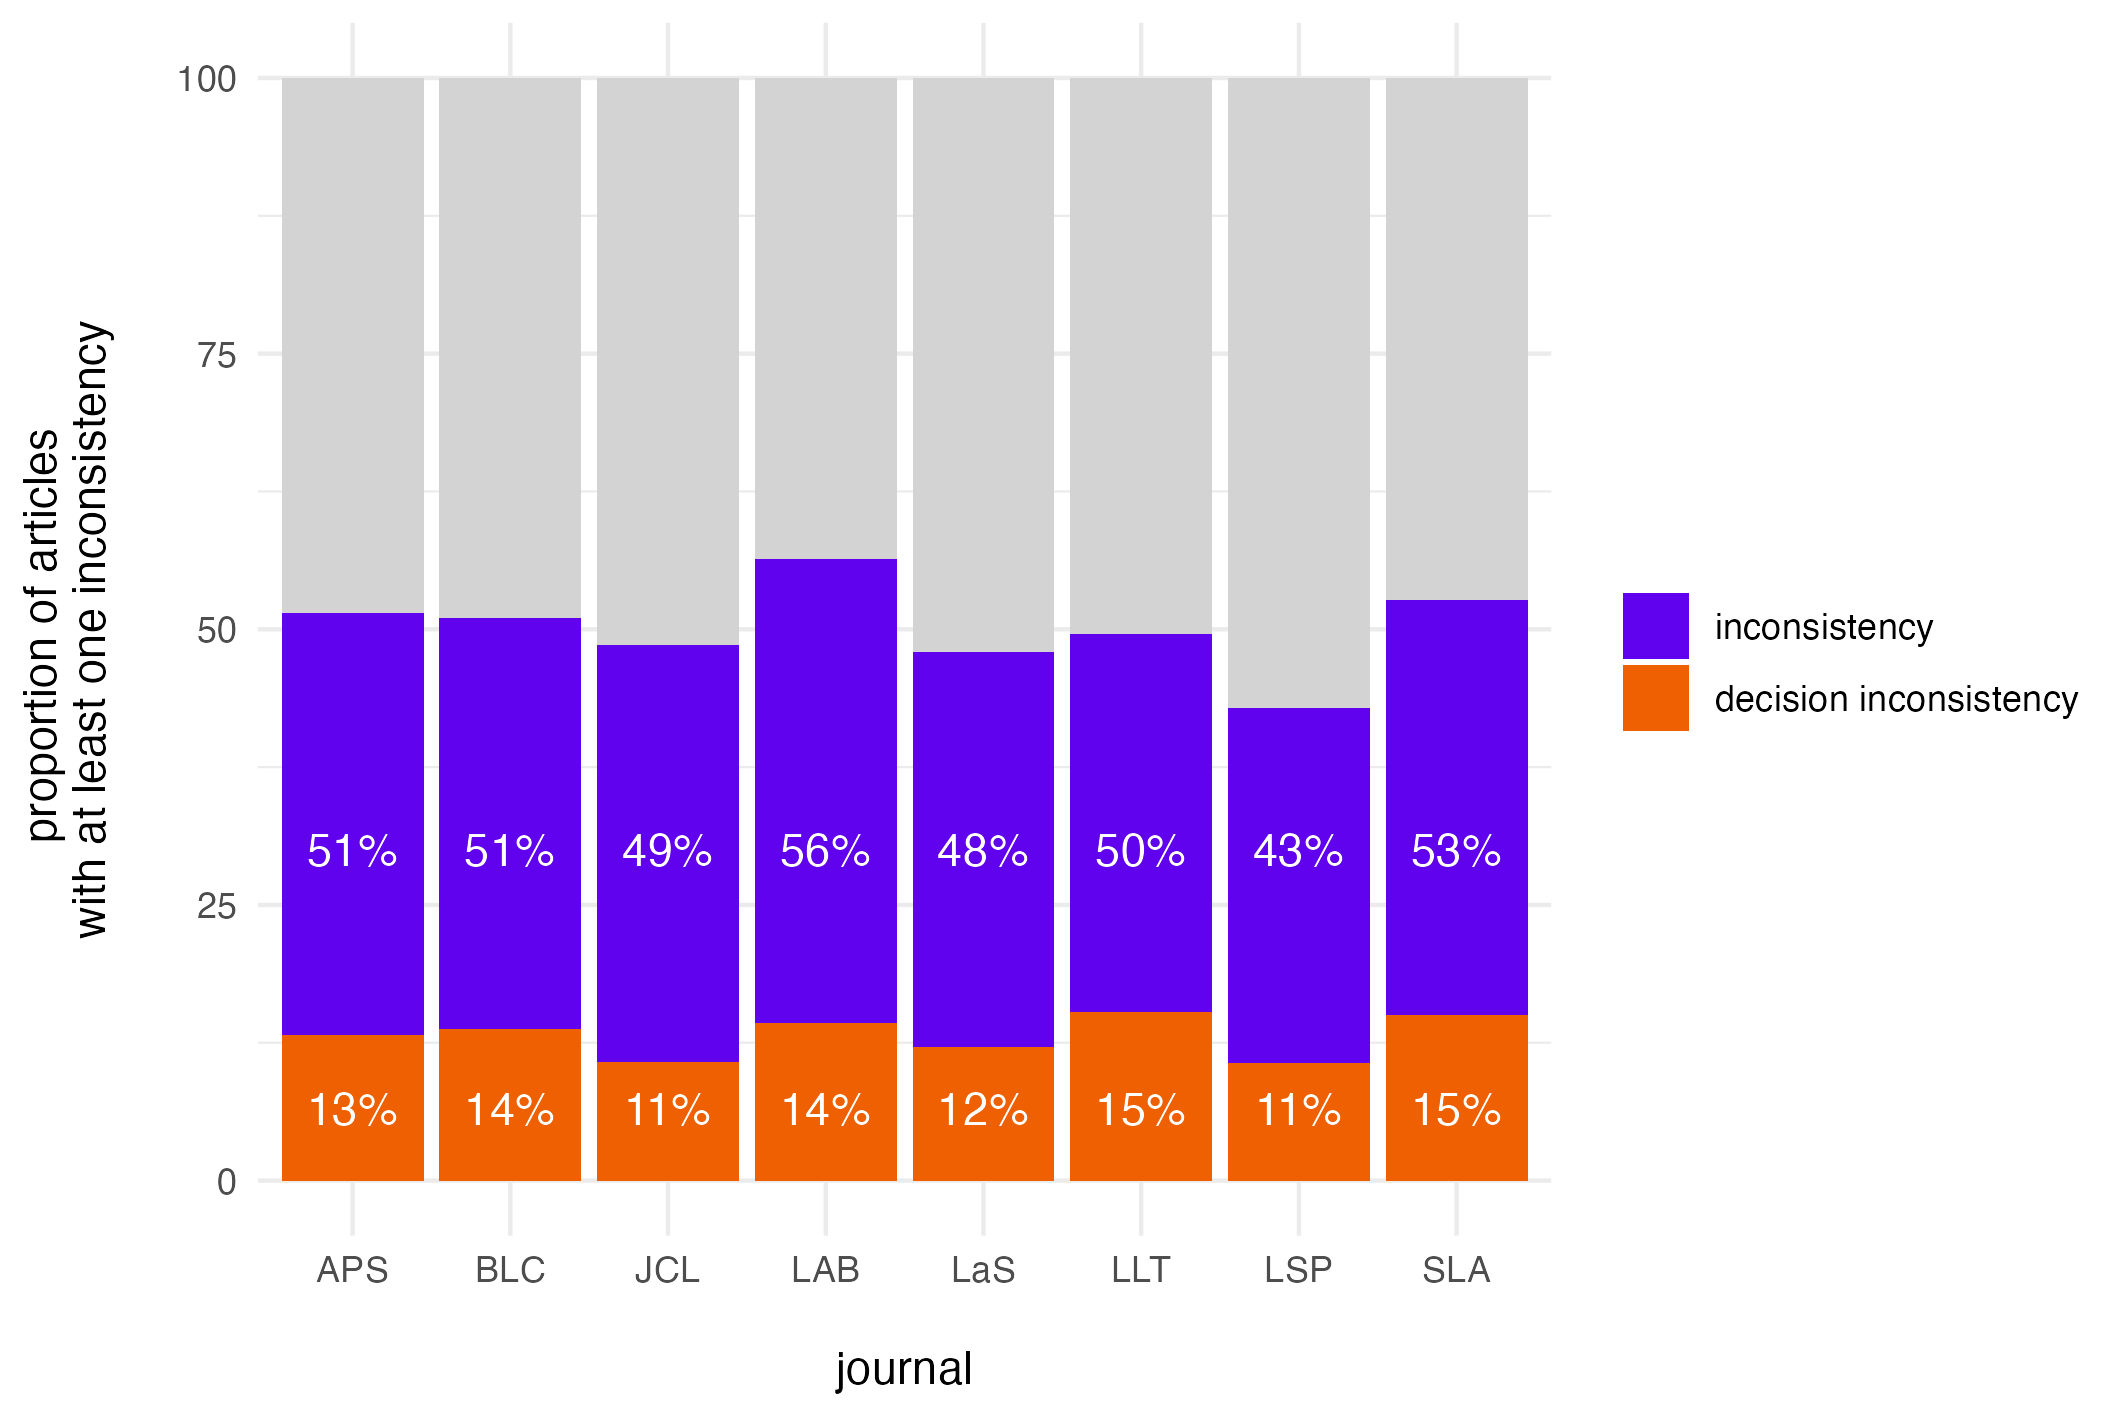
\includegraphics[width=1\textwidth,height=\textheight]{../plots/figure1.png}

}

\end{figure}%

\begin{figure}

\caption{\label{fig-year-prop}Proportion of inconsistencies / decision
inconsistencies from 2000 to 2023. Left: global rates with all journals
pooled; Right: rates per journal. Applied Psycholinguistics (APS),
Bilingualism: Language and Cognition (BLC), Linguistic Approaches to
Bilingualism (LAB), Language and Speech (LaS), Language Learning and
Techology (LLT), Journal of Language and Social Psychology (LSP),
Journal of Child Language (JCL), and Studies in Second Language
Acquisition (SLA).}

\centering{

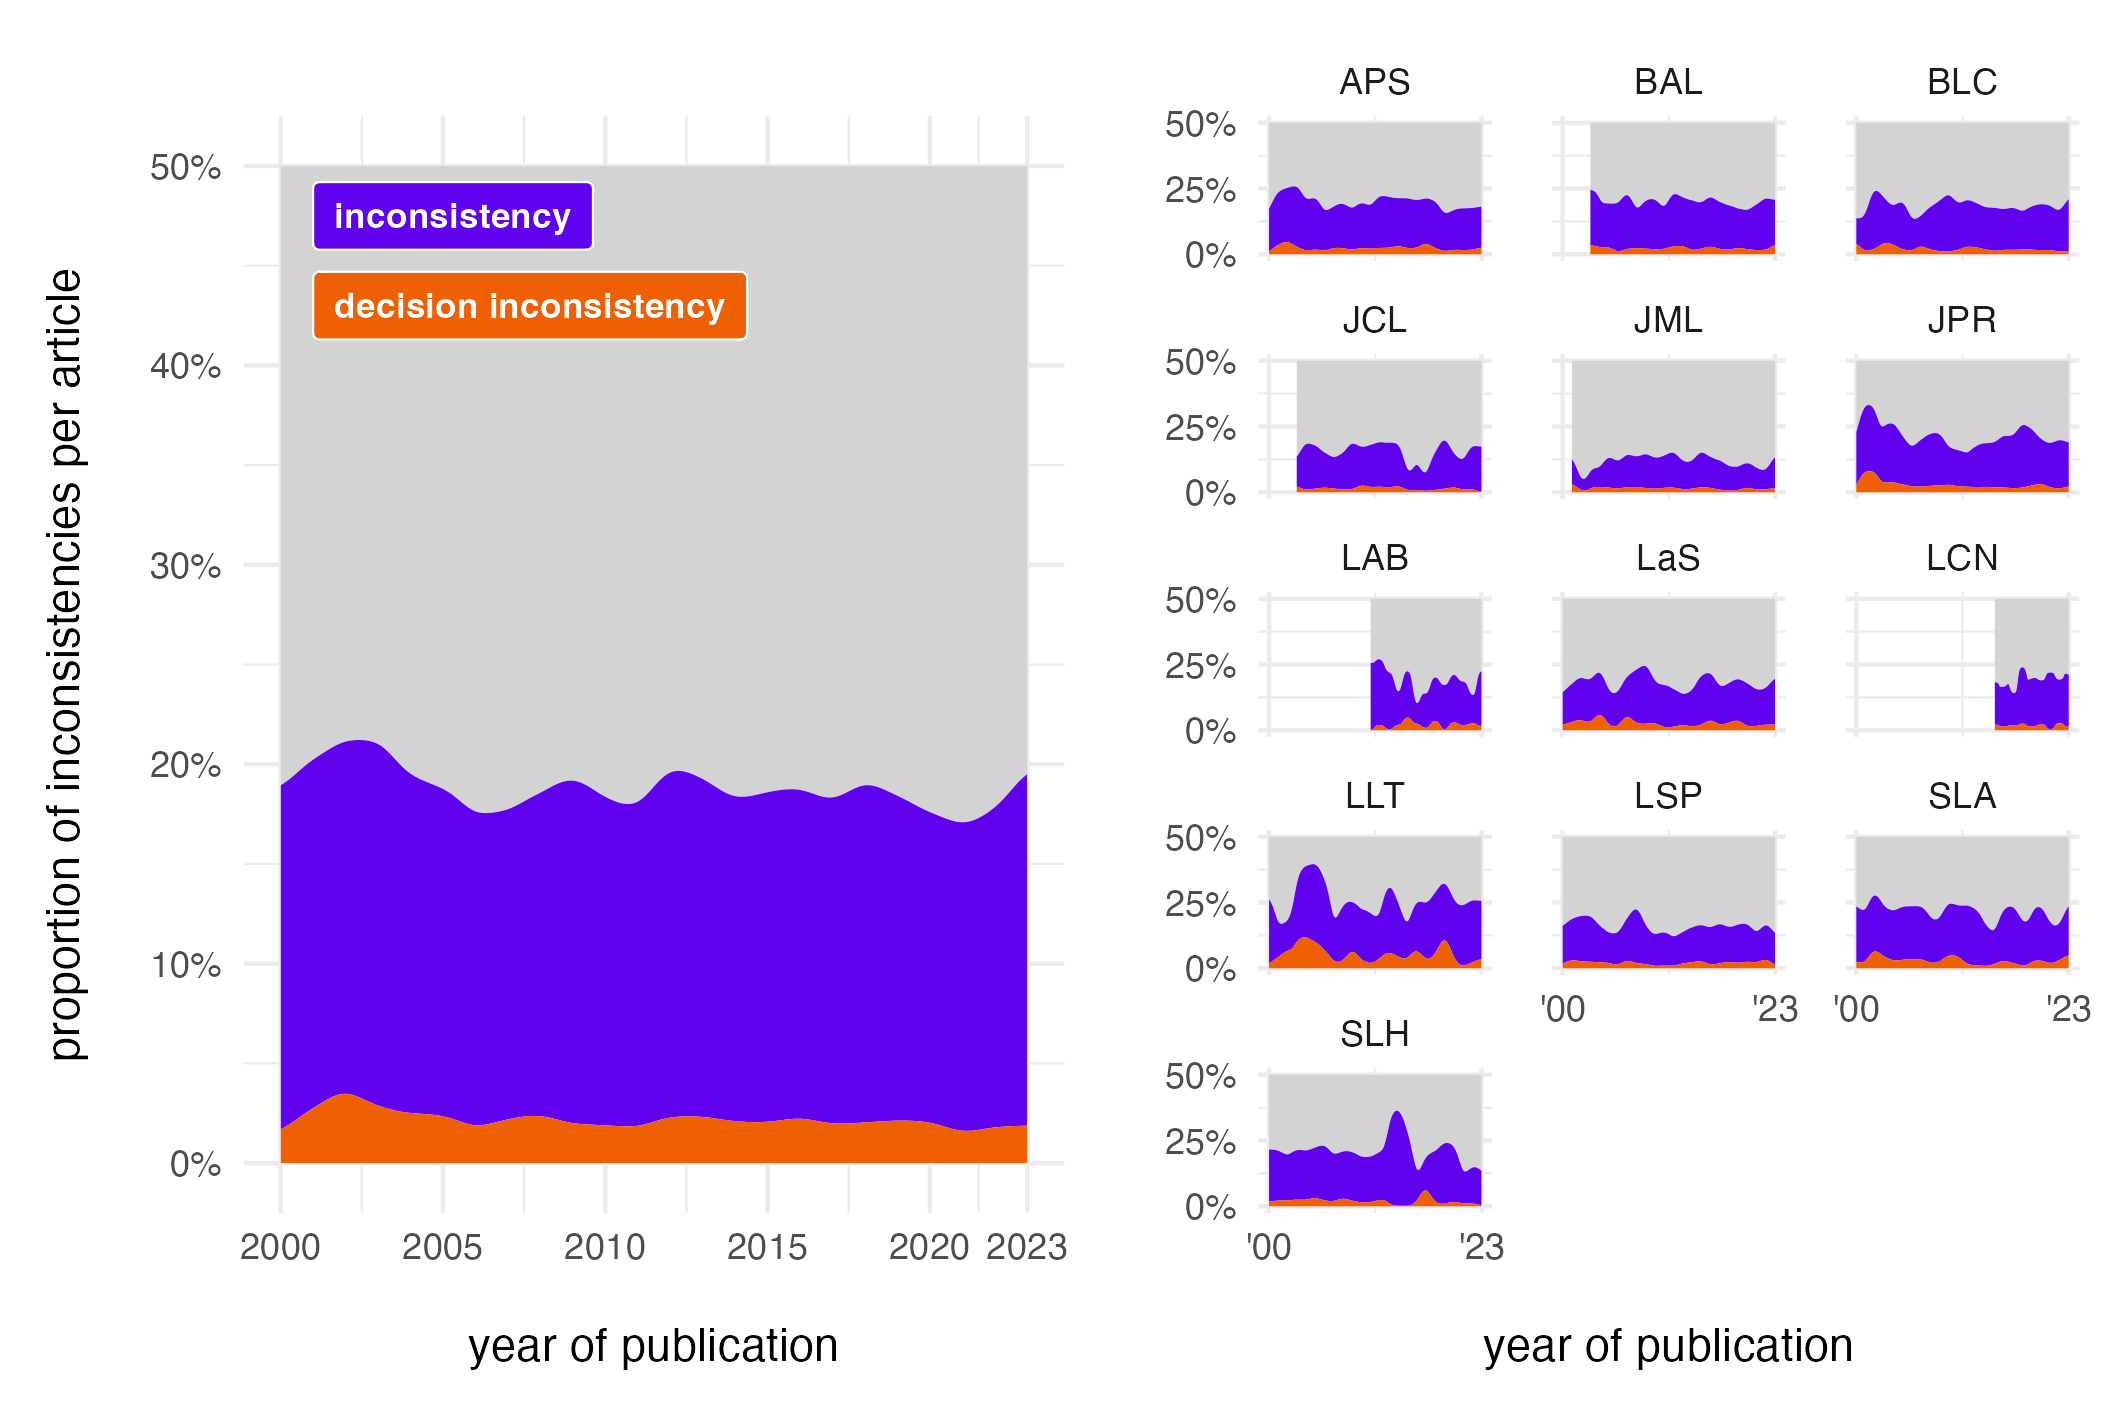
\includegraphics[width=1\textwidth,height=\textheight]{../plots/figure2.png}

}

\end{figure}%

When examining reported against recalculated p-values (see
Figure~\ref{fig-scatter}) for all inconsistencies, we can identify
certain spatial patterns (only inconsistencies that are based on `='
comparisons were included to make them easier to interpret, n = 5154 out
of 5166). First, the center of density of points is located in the
bottom left corner with more values reported closer to the alpha level.
This is not surprising, since there is a documented publication bias in
published quantitative articles, with hypotheses being much more often
confirmed (and thus p \textless{} .05) than not
(\citeproc{ref-franco2014publication}{Franco et al., 2014};
\citeproc{ref-sterling1959publication}{Sterling, 1959}). Second, there
is a linear density of points along the diagonal axis which corresponds
to numerically small inconsistencies, some of which might be related to
simple rounding errors. However, comparing the diagonal to the black
line, which represents a linear model predicting recalculated by
reported p-values, we can see a clear divergence of what is expected if
inconsistencies were equally likely in both directions
(i.e.~recalculated p-values were as likely to be smaller than the
reported p-value as larger). The slope of the regression line is flatter
than the diagonal axis which means that, on average, reported p-values
are lower than their recalculated counter parts. In other words,
inconsistencies have a tendency to lead to smaller p-values. This
potential bias can also be observed in decision inconsistencies. Of all
decisions inconsistencies (n = 655), 71\% represent cases in which a
reported significant result (p \textless{} 0.05) is recalculated as
non-significant value (p \textgreater{} 0.05).

\begin{figure}

\caption{\label{fig-scatter}Reported vs.~recalculated p-values for
inconsistencies that are based on `=' comparions. Black line
descriptively indicates the linear relationship, indicating a bias
towards lower reported p-values.}

\centering{

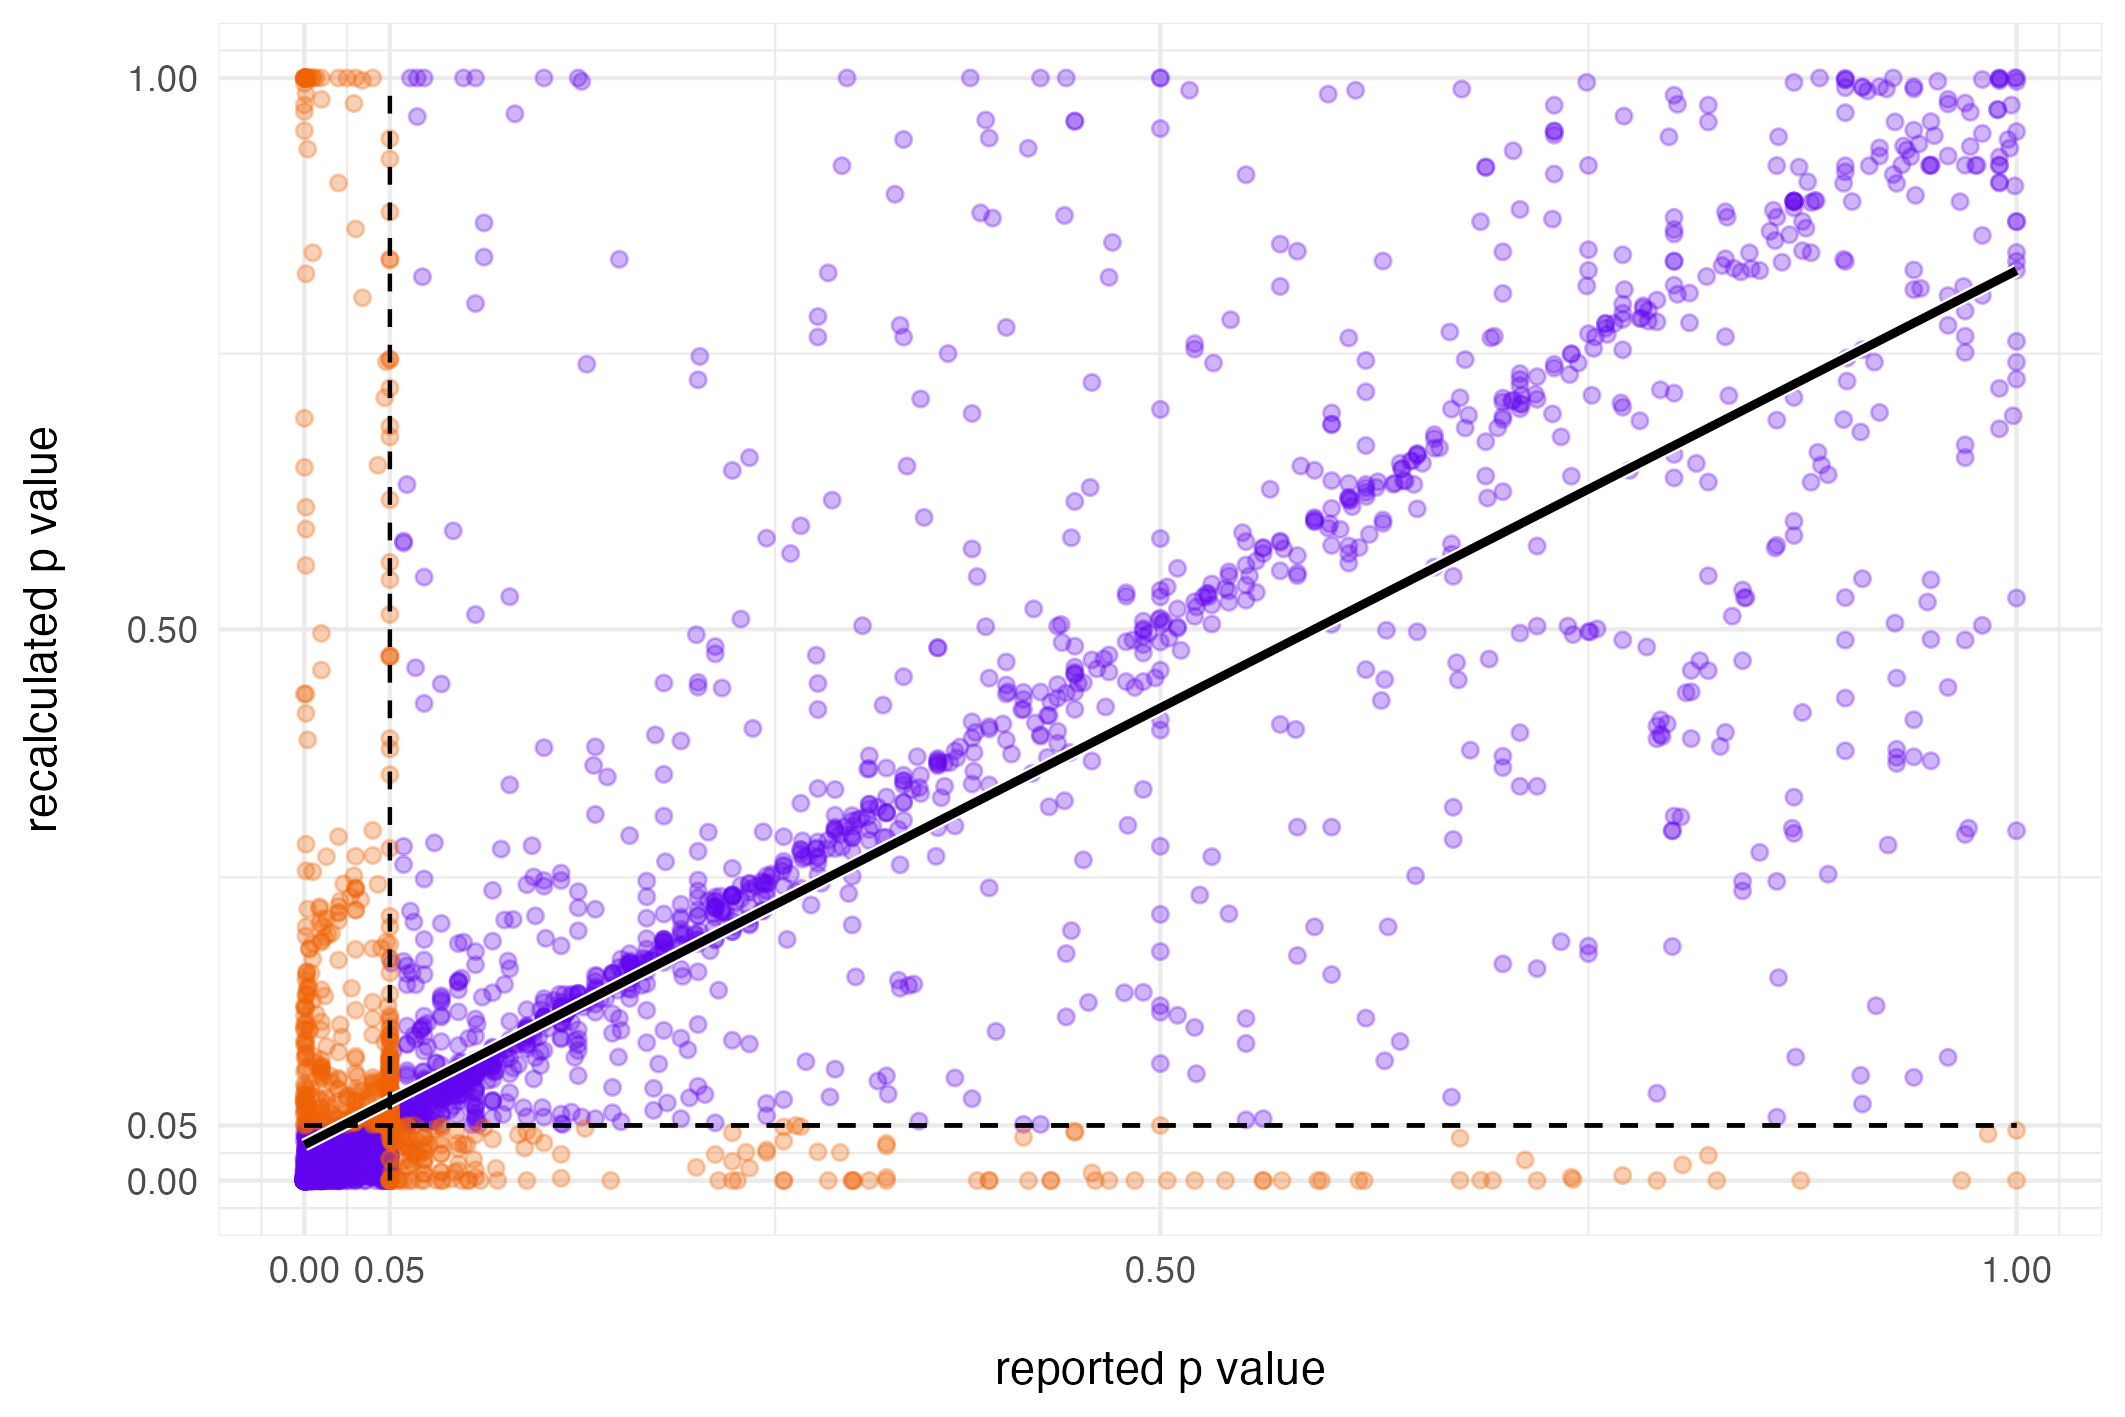
\includegraphics[width=1\textwidth,height=\textheight]{../plots/figure3.png}

}

\end{figure}%

\subsection{4.2 Manual inspection of decision
inconsistencies}\label{manual-inspection-of-decision-inconsistencies}

To further understand the nature of decision inconsistencies, we
manually inspected all of them (n=655). We (a) evaluated whether
statcheck has extracted the information correctly, and (b) assessed
whether the text actually suggest an erroneous inferential decision,
i.e.~whether the paper uses a reported significant result to claim a
significant effect or a reported non-significant result to claim a null
result.

\section{5. Discussion and
Recommendations}\label{discussion-and-recommendations}

\subsection{5.1. Statistical reporting inconsistencies are
prevalent}\label{statistical-reporting-inconsistencies-are-prevalent}

The present study found a concerning amount of statistical reporting
inconsistencies across a sample of 5804 experimental linguistic
articles, containing 3059 assessable p-values. 13.1\% of all p-values
were flagged as inconsistent and 1.7\% were flagged as decision
inconsistencies, i.e.~the reported p-value is on the opposite side of
the alpha threshold than the recalculated p-value. On average, 50\% of
assessable articles contained at least one inconsistency and 13\%
contained at least one decision inconsistency.

The present study can be considered a conceptual replication of previous
studies investigating statistical-reporting inconsistency in psychology
(\citeproc{ref-bakker2011mis}{Bakker \& Wicherts, 2011},
\citeproc{ref-bakker2014outlier}{2014};
\citeproc{ref-caperos2013consistency}{Caperos \& Pardo, 2013};
\citeproc{ref-claesen2023data}{Claesen et al., 2023};
\citeproc{ref-green2018statcheck}{Green et al., 2018};
\citeproc{ref-nuijten2016prevalence}{Nuijten et al., 2016};
\citeproc{ref-nuijten2020statcheck}{Nuijten \& Polanin, 2020};
\citeproc{ref-veldkamp2014statistical}{Veldkamp et al., 2014};
\citeproc{ref-wicherts2011willingness}{Wicherts et al., 2011}), medical
sciences (\citeproc{ref-garcia2004incongruence}{Garcı́a-Berthou \&
Alcaraz, 2004},; \citeproc{ref-van2023comparing}{Van Aert et al.,
2023}), psychiatry (\citeproc{ref-berle2007inconsistencies}{Berle \&
Starcevic, 2007}), cyber security
studies(\citeproc{ref-gross2021fidelity}{Groß, 2021}), technological
education research (\citeproc{ref-buckley2023estimating}{Buckley et al.,
2023}), and experimental philosophy
(\citeproc{ref-colombo2018statistical}{Colombo et al., 2018}). These
studies report on inconsistency rates between 4\% and 14\%, with between
10\% and 63\% of articles containing at least one inconsistency and
between 3\% and 21\% decision consistencies.

Even if the prevalence of these inconsistencies could be largely
attributed to inconsequential typos or rounding errors (an assumption we
cannot test without access to the data), the sheer amount of these
errors that have made it through peer-review should concern us. They are
human errors. If such a substantial amount of errors is found in plain
site, the question naturally arises how many errors that happen during
the data analysis itself remain undetected. If the tip of the iceberg
above water is so large, how large is the iceberg underneath the
surface?

The present examination also looked at whether the rates of
inconsistency changed over the last 23 years of publications.
Descriptive assessment did not indicate any noticeable trend. Moreover,
the rates of both inconsistencies and decision inconsistencies seem to
remain stable across journals.

Observed inconsistencies were characterized by reported p-values being
on average lower than their recalculated counterparts and the prevalence
of decision inconsistencies was higher for p-values reported as
significant than for those reported as non-significant. This could
indicate a systematic bias in favor of lower p-values in general and a
bias towards significant results in particular. Our data do not speak to
the causes of these biases, but possible reasons include the following:
Researchers might intentionally round down p-values because they think a
lower p-value is more convincing to reviewers and/or readers. This
practice has been admitted to by 1 in 5 surveyed psychological
researchers (\citeproc{ref-john2012measuring}{John et al., 2012}). Given
that quantitative linguists have been reported to commit questionable
research practices (and even fraud) more often than we would like to
(\citeproc{ref-isbell2022misconduct}{Isbell et al., 2022}), we cannot
exclude the possibility that some of the inconsistencies were
intentional. It is our strong belief, however, that the majority of
inconsistencies are unintentional.

Researchers might scrutinize non-significant results more than
significant results or fail to double check significant results more
often because results that confirm their hypothesis feed into their
confirmation bias (\citeproc{ref-nickerson1998confirmation}{Nickerson,
1998}). For example, Fugelsang et al.
(\citeproc{ref-fugelsang2004theory}{2004}) let researchers evaluate data
that are either consistent or inconsistent with their prior
expectations. They showed that when researchers encounter results that
disconfirm their expectations, they are likely to blame the methodology
while results that confirmed their expectations were rarely critically
scrutinized. Alternatively, the observed bias might be a reflection of
publication bias (\citeproc{ref-franco2014publication}{Franco et al.,
2014}; \citeproc{ref-sterling1959publication}{Sterling, 1959}) with
(erroneously) reported significant p-values being more likely to be
published than non-significant ones.

\subsection{5.2. Limitations of our
study}\label{limitations-of-our-study}

While we believe our work offers an important contribution to improving
statistical reporting practices in experimental linguistics, there are,
of course, a number of limitations. The present assessment and the
conclusions we can draw from them are limited. First, our sample is
limited to only a subset of experimental linguistic journals. Our sample
is based on a crude criterion of what constitutes an experimental
linguistic journal (see \citeproc{ref-kobrock2023assessing}{Kobrock \&
Roettger, 2023}) and we restricted ourselves further to (for us)
accessible journals which explicitly require APA statistical formatting
in the author guidelines. Thus it is possible that a different selection
of journals would have resulted in different results. However, given
that the inconsistency rates of our study are comparable to similar
studies from other disciplines and that the inconsistency rates are both
comparable across the eight journals and stable across the most recent
23 years, suggests that our findings are relevant for experimental
linguistics at large.

Second, given the constraints on automatically detecting test
statistics, statcheck misses reported values that either diverge from
APA reporting standards or are reported in tables. However,
inconsistency rates have been shown to be similar for results in APA
format vs.~results that diverge from APA formatting
(\citeproc{ref-bakker2011mis}{Bakker \& Wicherts, 2011};
\citeproc{ref-nuijten2016prevalence}{Nuijten et al., 2016}). Third,
statcheck slightly overestimates inconsistency rates, because it might
not accurately detect corrections for multiple comparisons
(\citeproc{ref-schmidt2017statcheck}{Schmidt, 2017}). Nuijten et al.
(\citeproc{ref-nuijten2017validity}{2017}), however, show that not only
were there only a small proportion of flagged inconsistencies related to
multiple comparisons, but also that these multiple comparisons
themselves were often erroneously reported. They conclude that
``{[}a{]}ny reporting inconsistencies associated with these tests and
corrections could not explain the high prevalence of reporting
inconsistencies'' (\citeproc{ref-nuijten2017validity}{Nuijten et al.,
2017, p. 27}). More elaborate automatic tools for the extraction of
statistical information might allow a more detailed and more accurate
assessment of statistical reporting in the future (e.g.
\citeproc{ref-kalmbach2023rule}{Kalmbach et al., 2023}). But even
statcheck is limited and only provides a rough proxy of true
inconsistency rate in the published literature, we hope the reader
agrees that it is a state of affairs that should be tackled.

\subsection{5.3. Recommendations for the
field}\label{recommendations-for-the-field}

There are concrete actionable steps the field of experimental
linguistics can make to reduce statistical reporting inconsistencies. In
order to avoid simple copy and paste errors related to working in two
separate programs for writing the manuscript and conducting the
statistical analysis, authors should consider `literate programming',
i.e.~an integration of analysis code and prose into a single, dynamic
document (\citeproc{ref-casillas2023opening}{Casillas et al., 2023};
\citeproc{ref-knuth1984literate}{Knuth, 1984}). Several implementations
of literate programming are freely available to researchers including
common R markdown files (Rmd) and Quarto markdown files (qmd). Literate
programming can ensure that values derived by the statistical analysis
is automatically integrated into the manuscript document, avoiding
errors that might happen during a transfer from one program to the
other.

Authors should also consider sharing their derived data (i.e.~the
anonymized data table that was analyzed) as well as a detailed
description of their statistical protocol, ideally in form of
reproducible scripts. Sharing reproducible analyses with reviewers
allows the reviewers the reproduce the authors' analyses, possibly
detect errors or even inappropriate statistical choices before
publication, thus improving the quality of their work. Moreover,
publicly sharing their analyses has numerous benefits to the authors
themselves beyond error detection: Open data and materials can
facilitate collaboration (\citeproc{ref-boland2017ten}{Boland et al.,
2017}), increase efficiency and sustainability
(\citeproc{ref-lowndes2017our}{Lowndes et al., 2017}), and are cited
more often (\citeproc{ref-colavizza2020citation}{Colavizza et al.,
2020}).

If authors do not share data and scripts, reviewers can check at least
the statistical reporting consistency in the manuscript by using tools
such as statcheck (\citeproc{ref-nuijten2023statcheck}{Nuijten \&
Epskamp, 2023}, http://statcheck.io) or p-checker
(\citeproc{ref-schonbrodt2015p}{Schönbrodt, 2015},
http://shinyapps.org/apps/p-checker/). Reviewers could consider consider
requesting data and scripts during peer review. Such requests might be
particularly justified when inconsistencies are apparent. Explicitly
requesting to share data might already instill additional care and
quality checks when authors prepare their materials, but also allows the
reviewers to carefully reproduce the results, and critically evaluate
all choices made in the statistical analysis
(\citeproc{ref-sakaluk2014analytic}{Sakaluk et al., 2014}). Recent
evidence suggest experimental linguistics are still characterized by a
pluralism of statistical approaches, even when trying to answer the same
research question (\citeproc{ref-coretta_multidimensional_2023}{Coretta
et al., 2023}). Some of these approaches are might be more appropriate
than others (\citeproc{ref-sondereggera2024advancements}{Sonderegger \&
Sóskuthy, 2024}; \citeproc{ref-vasishth2023some}{Vasishth, 2023}), so
more thorough evaluations of how researchers arrive at their statistical
conclusions might elevate their analytical robustness.

Journal editors could explicitly recommend consistency checks with apps
such as statcheck during peer review, a practice that has been taken up
on by several journals from neighboring disciplines (Psychological
Science\footnote{http://www.psychologicalscience.org/publications/psychological\_science/ps-submissions;
  accessed on July 15, 2024.}, Advances in Methods and Practices in
Psychological Science\footnote{https://www.psychologicalscience.org/publications/ampps/ampps-submission-guidelines;
  accessed on on July 15, 2024.}, Stress \& Health
\citeproc{ref-barber2017meticulous}{Barber, 2017}). Editors could also
demand, recommend or at least encourage data sharing for publication in
their journal. Data sharing policies have been shown to substantially
increase the reproducibility of analyses
(\citeproc{ref-hardwicke2018data}{Hardwicke et al., 2018}; e.g.
\citeproc{ref-laurinavichyute2022share}{Laurinavichyute et al., 2022}).

\section{References}\label{references}

\phantomsection\label{refs}
\begin{CSLReferences}{1}{0}
\bibitem[\citeproctext]{ref-APA2020}
American Psychological Association. (2020). \emph{Publication manual of
the {American Psychological Association}} (7th ed.). Author.
\url{https://doi.org/10.1037/0000173-000}

\bibitem[\citeproctext]{ref-arvan2022reproducibility}
Arvan, M., Pina, L., \& Parde, N. (2022). Reproducibility in
computational linguistics: Is source code enough? \emph{Proceedings of
the 2022 Conference on Empirical Methods in Natural Language
Processing}, 2350--2361.

\bibitem[\citeproctext]{ref-bakker2011mis}
Bakker, M., \& Wicherts, J. M. (2011). The (mis) reporting of
statistical results in psychology journals. \emph{Behavior Research
Methods}, \emph{43}, 666--678.

\bibitem[\citeproctext]{ref-bakker2014outlier}
Bakker, M., \& Wicherts, J. M. (2014). Outlier removal and the relation
with reporting errors and quality of psychological research. \emph{PloS
One}, \emph{9}(7), e103360.

\bibitem[\citeproctext]{ref-barber2017meticulous}
Barber, L. K. (2017). Meticulous manuscripts, messy results: Working
together for robust science reporting. \emph{Stress \& Health},
\emph{33}(2), 89--91.

\bibitem[\citeproctext]{ref-berle2007inconsistencies}
Berle, D., \& Starcevic, V. (2007). Inconsistencies between reported
test statistics and p-values in two psychiatry journals.
\emph{International Journal of Methods in Psychiatric Research},
\emph{16}(4), 202--207.

\bibitem[\citeproctext]{ref-bochynska2023reproducible}
Bochynska, A., Keeble, L., Halfacre, C., Casillas, J. V., Champagne,
I.-A., Chen, K., Röthlisberger, M., Buchanan, E. M., \& Roettger, T.
(2023). Reproducible research practices and transparency across
linguistics. \emph{Glossa Psycholinguistics}, \emph{2}(1).

\bibitem[\citeproctext]{ref-boland2017ten}
Boland, M. R., Karczewski, K. J., \& Tatonetti, N. P. (2017). Ten simple
rules to enable multi-site collaborations through data sharing. In
\emph{PLoS computational biology} (1; Vol. 13, p. e1005278). Public
Library of Science San Francisco, CA USA.

\bibitem[\citeproctext]{ref-buckley2023estimating}
Buckley, J., Hyland, T., \& Seery, N. (2023). Estimating the
replicability of technology education research. \emph{International
Journal of Technology and Design Education}, \emph{33}(4), 1243--1264.

\bibitem[\citeproctext]{ref-caperos2013consistency}
Caperos, J. M., \& Pardo, A. (2013). Consistency errors in p-values
reported in spanish psychology journals. \emph{Psicothema},
\emph{25}(3), 408--414.

\bibitem[\citeproctext]{ref-casillas2023opening}
Casillas, J. V., Constantin-Dureci, G., Rascón, I. A., Shao, J.,
Rodrı́guez, S. A., Gadamsetty, A., Minetti, A., Laungani, K., Thatcher,
J., Gardere, R.-T., et al. (2023). \emph{Opening open science to all:
Demystifying reproducibility and transparency practices in linguistic
research}.

\bibitem[\citeproctext]{ref-claesen2023data}
Claesen, A., Vanpaemel, W., Maerten, A.-S., Verliefde, T., Tuerlinckx,
F., \& Heyman, T. (2023). Data sharing upon request and statistical
consistency errors in psychology: A replication of wicherts, bakker and
molenaar (2011). \emph{Plos One}, \emph{18}(4), e0284243.

\bibitem[\citeproctext]{ref-colavizza2020citation}
Colavizza, G., Hrynaszkiewicz, I., Staden, I., Whitaker, K., \&
McGillivray, B. (2020). The citation advantage of linking publications
to research data. \emph{PloS One}, \emph{15}(4), e0230416.

\bibitem[\citeproctext]{ref-colombo2018statistical}
Colombo, M., Duev, G., Nuijten, M. B., \& Sprenger, J. (2018).
Statistical reporting inconsistencies in experimental philosophy.
\emph{PloS One}, \emph{13}(4), e0194360.

\bibitem[\citeproctext]{ref-coretta_multidimensional_2023}
Coretta, S., Casillas, J. V., Roessig, S., Franke, M., Ahn, B.,
Al-Hoorie, A. H., Al-Tamimi, J., Alotaibi, N. E., AlShakhori, M. K.,
Altmiller, R. M., Arantes, P., Athanasopoulou, A., Baese-Berk, M. M.,
Bailey, G., Sangma, C. B. A., Beier, E. J., Benavides, G. M., Benker,
N., BensonMeyer, E. P., \ldots{} Roettger, T. B. (2023).
Multidimensional {Signals} and {Analytic} {Flexibility}: {Estimating}
{Degrees} of {Freedom} in {Human}-{Speech} {Analyses}. \emph{Advances in
Methods and Practices in Psychological Science}, \emph{6}(3),
25152459231162567. \url{https://doi.org/10.1177/25152459231162567}

\bibitem[\citeproctext]{ref-franco2014publication}
Franco, A., Malhotra, N., \& Simonovits, G. (2014). Publication bias in
the social sciences: Unlocking the file drawer. \emph{Science},
\emph{345}(6203), 1502--1505.

\bibitem[\citeproctext]{ref-fugelsang2004theory}
Fugelsang, J. A., Stein, C. B., Green, A. E., \& Dunbar, K. N. (2004).
Theory and data interactions of the scientific mind: Evidence from the
molecular and the cognitive laboratory. \emph{Canadian Journal of
Experimental Psychology/Revue Canadienne de Psychologie
Exp{é}rimentale}, \emph{58}(2), 86.

\bibitem[\citeproctext]{ref-garcia2004incongruence}
Garcı́a-Berthou, E., \& Alcaraz, C. (2004). Incongruence between test
statistics and p values in medical papers. \emph{BMC Medical Research
Methodology}, \emph{4}, 1--5.

\bibitem[\citeproctext]{ref-green2018statcheck}
Green, C. D., Abbas, S., Belliveau, A., Beribisky, N., Davidson, I. J.,
DiGiovanni, J., Heidari, C., Martin, S. M., Oosenbrug, E., \&
Wainewright, L. M. (2018). Statcheck in canada: What proportion of CPA
journal articles contain errors in the reporting of p-values?
\emph{Canadian Psychology/Psychologie Canadienne}, \emph{59}(3), 203.

\bibitem[\citeproctext]{ref-gross2021fidelity}
Groß, T. (2021). Fidelity of statistical reporting in 10 years of cyber
security user studies. \emph{Socio-Technical Aspects in Security and
Trust: 9th International Workshop, STAST 2019, Luxembourg City,
Luxembourg, September 26, 2019, Revised Selected Papers 9}, 3--26.

\bibitem[\citeproctext]{ref-hardwicke2018data}
Hardwicke, T. E., Mathur, M. B., MacDonald, K., Nilsonne, G., Banks, G.
C., Kidwell, M. C., Hofelich Mohr, A., Clayton, E., Yoon, E. J., Henry
Tessler, M., et al. (2018). Data availability, reusability, and analytic
reproducibility: Evaluating the impact of a mandatory open data policy
at the journal cognition. \emph{Royal Society Open Science},
\emph{5}(8), 180448.

\bibitem[\citeproctext]{ref-isbell2022misconduct}
Isbell, D. R., Brown, D., Chen, M., Derrick, D. J., Ghanem, R., Arvizu,
M. N. G., Schnur, E., Zhang, M., \& Plonsky, L. (2022). Misconduct and
questionable research practices: The ethics of quantitative data
handling and reporting in applied linguistics. \emph{The Modern Language
Journal}, \emph{106}(1), 172--195.

\bibitem[\citeproctext]{ref-john2012measuring}
John, L. K., Loewenstein, G., \& Prelec, D. (2012). Measuring the
prevalence of questionable research practices with incentives for truth
telling. \emph{Psychological Science}, \emph{23}(5), 524--532.

\bibitem[\citeproctext]{ref-kalmbach2023rule}
Kalmbach, T., Hoffmann, M., Lell, N., \& Scherp, A. (2023). On the
rule-based extraction of statistics reported in scientific papers.
\emph{International Conference on Applications of Natural Language to
Information Systems}, 326--338.

\bibitem[\citeproctext]{ref-knuth1984literate}
Knuth, D. E. (1984). Literate programming. \emph{The Computer Journal},
\emph{27}(2), 97--111.

\bibitem[\citeproctext]{ref-kobrock2023assessing}
Kobrock, K., \& Roettger, T. (2023). Assessing the replication landscape
in experimental linguistics. \emph{Glossa Psycholinguistics},
\emph{2}(1), 1--28.

\bibitem[\citeproctext]{ref-laurinavichyute2022share}
Laurinavichyute, A., Yadav, H., \& Vasishth, S. (2022). Share the code,
not just the data: A case study of the reproducibility of articles
published in the journal of memory and language under the open data
policy. \emph{Journal of Memory and Language}, \emph{125}, 104332.

\bibitem[\citeproctext]{ref-lowndes2017our}
Lowndes, J. S. S., Best, B. D., Scarborough, C., Afflerbach, J. C.,
Frazier, M. R., O'Hara, C. C., Jiang, N., \& Halpern, B. S. (2017). Our
path to better science in less time using open data science tools.
\emph{Nature Ecology \& Evolution}, \emph{1}(6), 0160.

\bibitem[\citeproctext]{ref-nickerson1998confirmation}
Nickerson, R. S. (1998). Confirmation bias: A ubiquitous phenomenon in
many guises. \emph{Review of General Psychology}, \emph{2}(2), 175--220.

\bibitem[\citeproctext]{ref-nuijten2017validity}
Nuijten, M. B., Assen, M. A. van, Hartgerink, C., Epskamp, S., \&
Wicherts, J. M. (2017). \emph{The validity of the tool {``statcheck''}
in discovering statistical reporting inconsistencies}.

\bibitem[\citeproctext]{ref-nuijten2023statcheck}
Nuijten, M. B., \& Epskamp, S. (2023). \emph{Statcheck: Extract
statistics from articles and recompute p-values(1.4. 1-beta. 2){[}r{]}}.

\bibitem[\citeproctext]{ref-nuijten2016prevalence}
Nuijten, M. B., Hartgerink, C. H., Van Assen, M. A., Epskamp, S., \&
Wicherts, J. M. (2016). The prevalence of statistical reporting errors
in psychology (1985--2013). \emph{Behavior Research Methods}, \emph{48},
1205--1226.

\bibitem[\citeproctext]{ref-nuijten2020statcheck}
Nuijten, M. B., \& Polanin, J. R. (2020). {``Statcheck''}: Automatically
detect statistical reporting inconsistencies to increase reproducibility
of meta-analyses. \emph{Research Synthesis Methods}, \emph{11}(5),
574--579.

\bibitem[\citeproctext]{ref-roettger2019researcher}
Roettger, T. B. (2019). Researcher degrees of freedom in phonetic
research. \emph{Laboratory Phonology}, \emph{10}(1).

\bibitem[\citeproctext]{ref-sakaluk2014analytic}
Sakaluk, J., Williams, A., \& Biernat, M. (2014). Analytic review as a
solution to the misreporting of statistical results in psychological
science. \emph{Perspectives on Psychological Science}, \emph{9}(6),
652--660.

\bibitem[\citeproctext]{ref-schmidt2017statcheck}
Schmidt, T. (2017). \emph{Statcheck does not work: All the numbers.
Reply to nuijten et al.(2017)}.

\bibitem[\citeproctext]{ref-schonbrodt2015p}
Schönbrodt, F. D. (2015). \emph{P-checker: One-for-all p-value
analyzer}. \url{http://shinyapps.org/apps/p-checker/}.

\bibitem[\citeproctext]{ref-sondereggera2024advancements}
Sonderegger, M., \& Sóskuthy, M. (2024). \emph{Advancements of phonetics
in the 21st century: Quantitative data analysis}.

\bibitem[\citeproctext]{ref-sterling1959publication}
Sterling, T. D. (1959). Publication decisions and their possible effects
on inferences drawn from tests of significance---or vice versa.
\emph{Journal of the American Statistical Association}, \emph{54}(285),
30--34.

\bibitem[\citeproctext]{ref-van2023comparing}
Van Aert, R. C., Nuijten, M. B., Olsson-Collentine, A., Stoevenbelt, A.
H., Van Den Akker, O. R., Klein, R. A., \& Wicherts, J. M. (2023).
Comparing the prevalence of statistical reporting inconsistencies in
COVID-19 preprints and matched controls: A registered report.
\emph{Royal Society Open Science}, \emph{10}(8), 202326.

\bibitem[\citeproctext]{ref-vasishth2023some}
Vasishth, S. (2023). Some right ways to analyze (psycho) linguistic
data. \emph{Annual Review of Linguistics}, \emph{9}(1), 273--291.

\bibitem[\citeproctext]{ref-veldkamp2014statistical}
Veldkamp, C. L., Nuijten, M. B., Dominguez-Alvarez, L., Van Assen, M.
A., \& Wicherts, J. M. (2014). Statistical reporting errors and
collaboration on statistical analyses in psychological science.
\emph{PloS One}, \emph{9}(12), e114876.

\bibitem[\citeproctext]{ref-wicherts2011willingness}
Wicherts, J. M., Bakker, M., \& Molenaar, D. (2011). Willingness to
share research data is related to the strength of the evidence and the
quality of reporting of statistical results. \emph{PloS One},
\emph{6}(11), e26828.

\end{CSLReferences}

\appendix

\section{Title for Appendix}\label{title-for-appendix}






\end{document}
